\subsection{Graphical Interface Interaction}

		A graphical web interface was chosen as solution to give users a quick
		interaction with \TVB . The web interface is easy to access (local or
		remotely) through a web browser, it can be used by different types of
		users, including those without programming knowledge, and it offers
		great support while learning about \TVB concepts and workflow
		expectations.  In our architecture diagrams, the actor accessing \TVB
		through the web interface is called a \emph{G-User}.

		The http is served using \emph{Cherrypy}
		\texttt{http://www.cherrypy.org/} which is a minimalist, object-
		oriented web framework,  in combination with \emph{Genshi} templating
		system, to support the separation of layers as guided by \emph{MVC
		(Model View Controller)} pattern.

		\subsubsection{Projects, Accounts, Operations \& Data}

		TVB uses entities like: Account, Project, Operation, DataType and
		Workflow, for modeling G-User actions and artifacts.

 \begin{figure}[!htbp]

		\centering
		\subfloat[][]{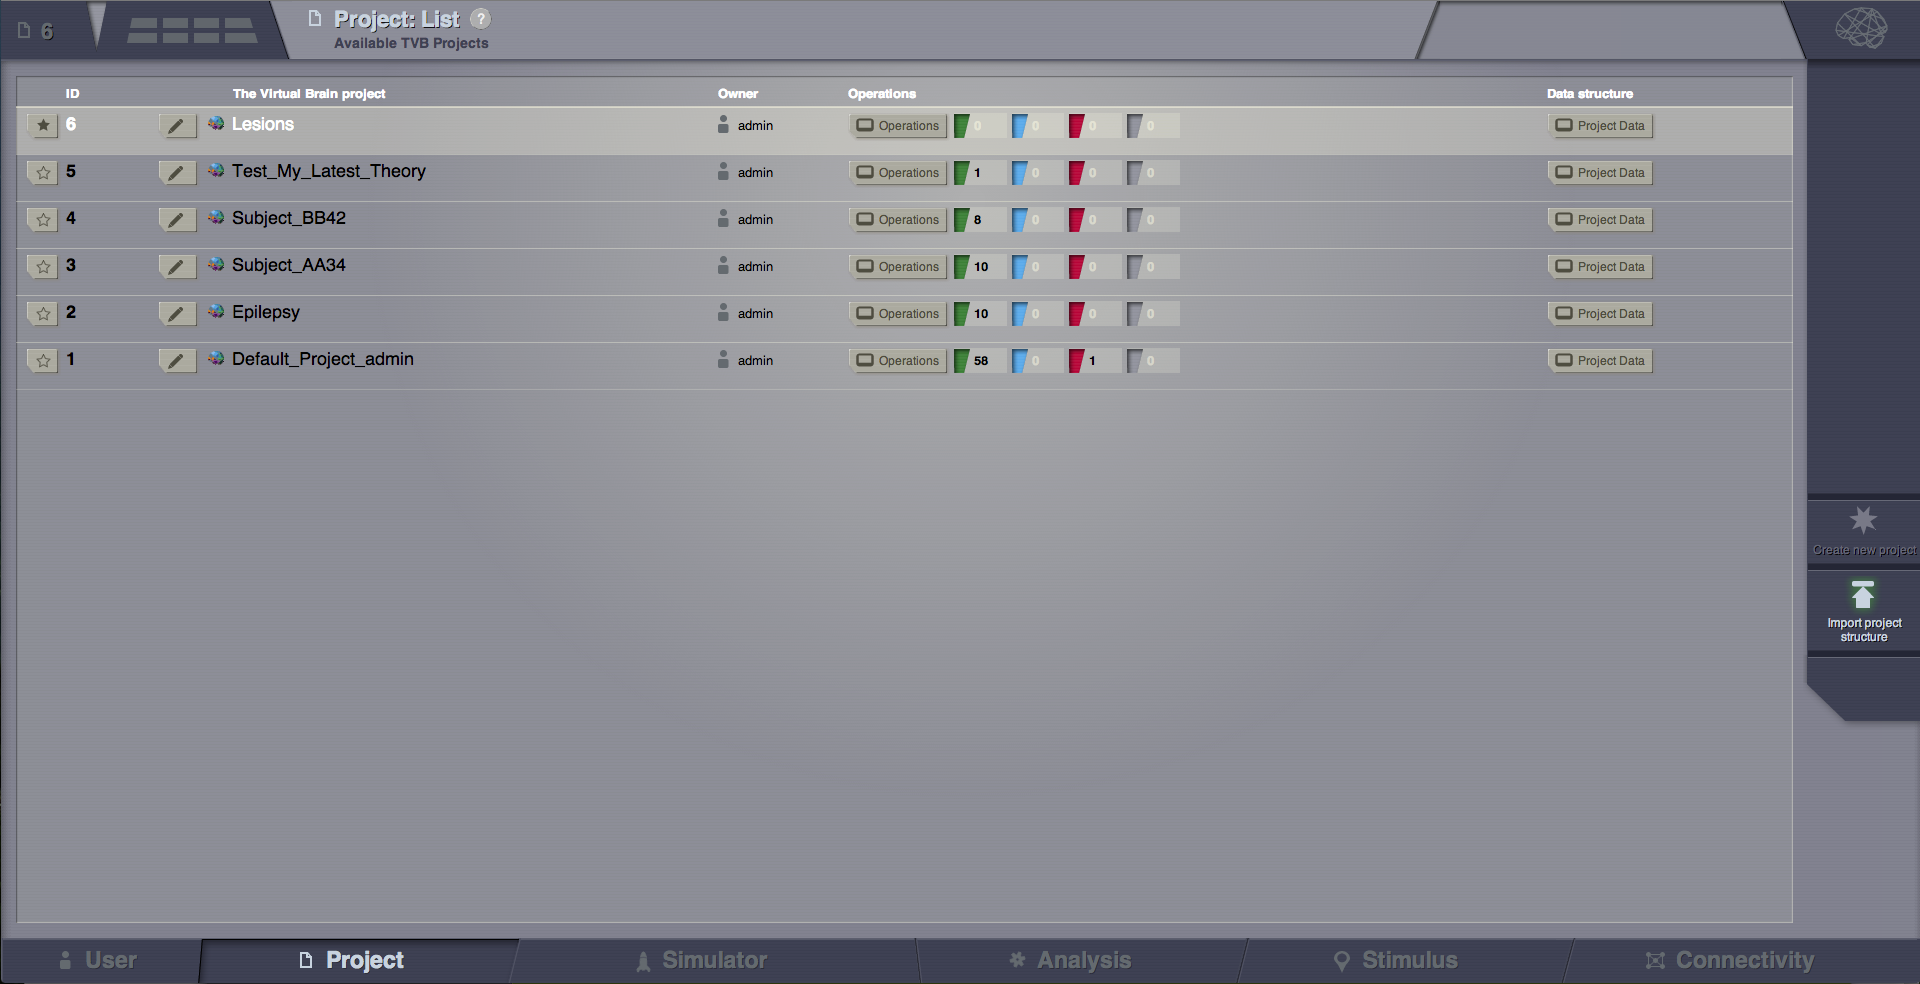
\includegraphics[width=0.47\textwidth]{images/ui_projects.png}}
		\\
		\subfloat[][]{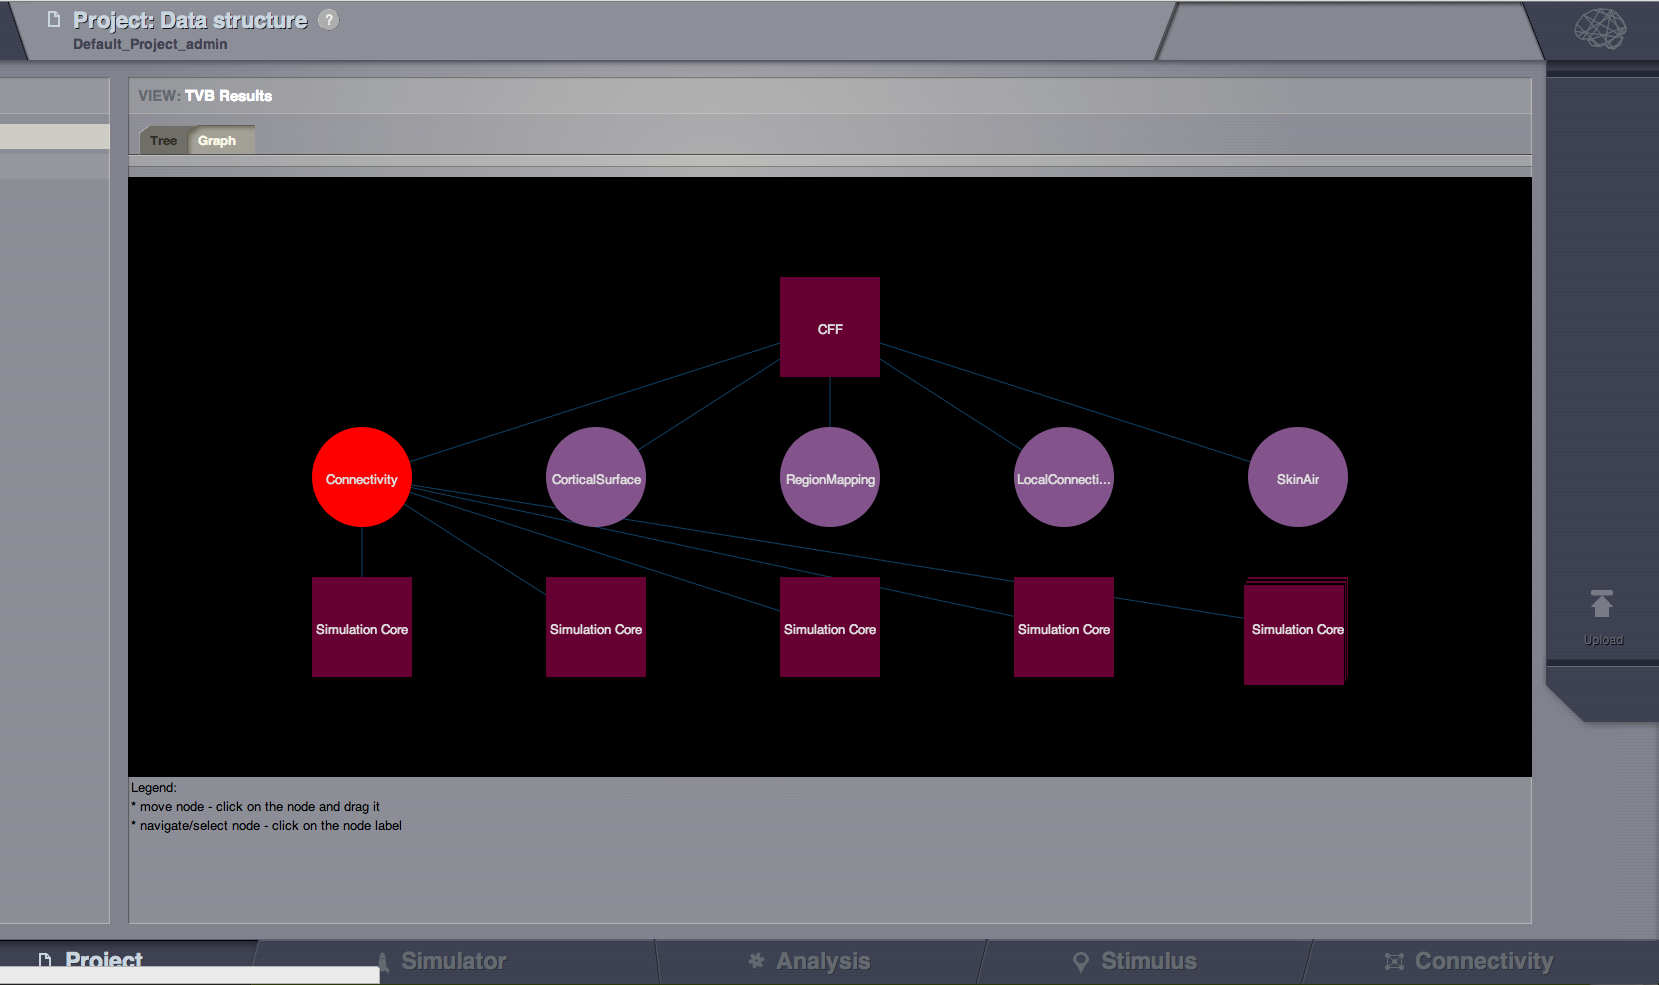
\includegraphics[width=0.47\textwidth]{images/ui_project_graph.png}}
		\\
		\subfloat[][]{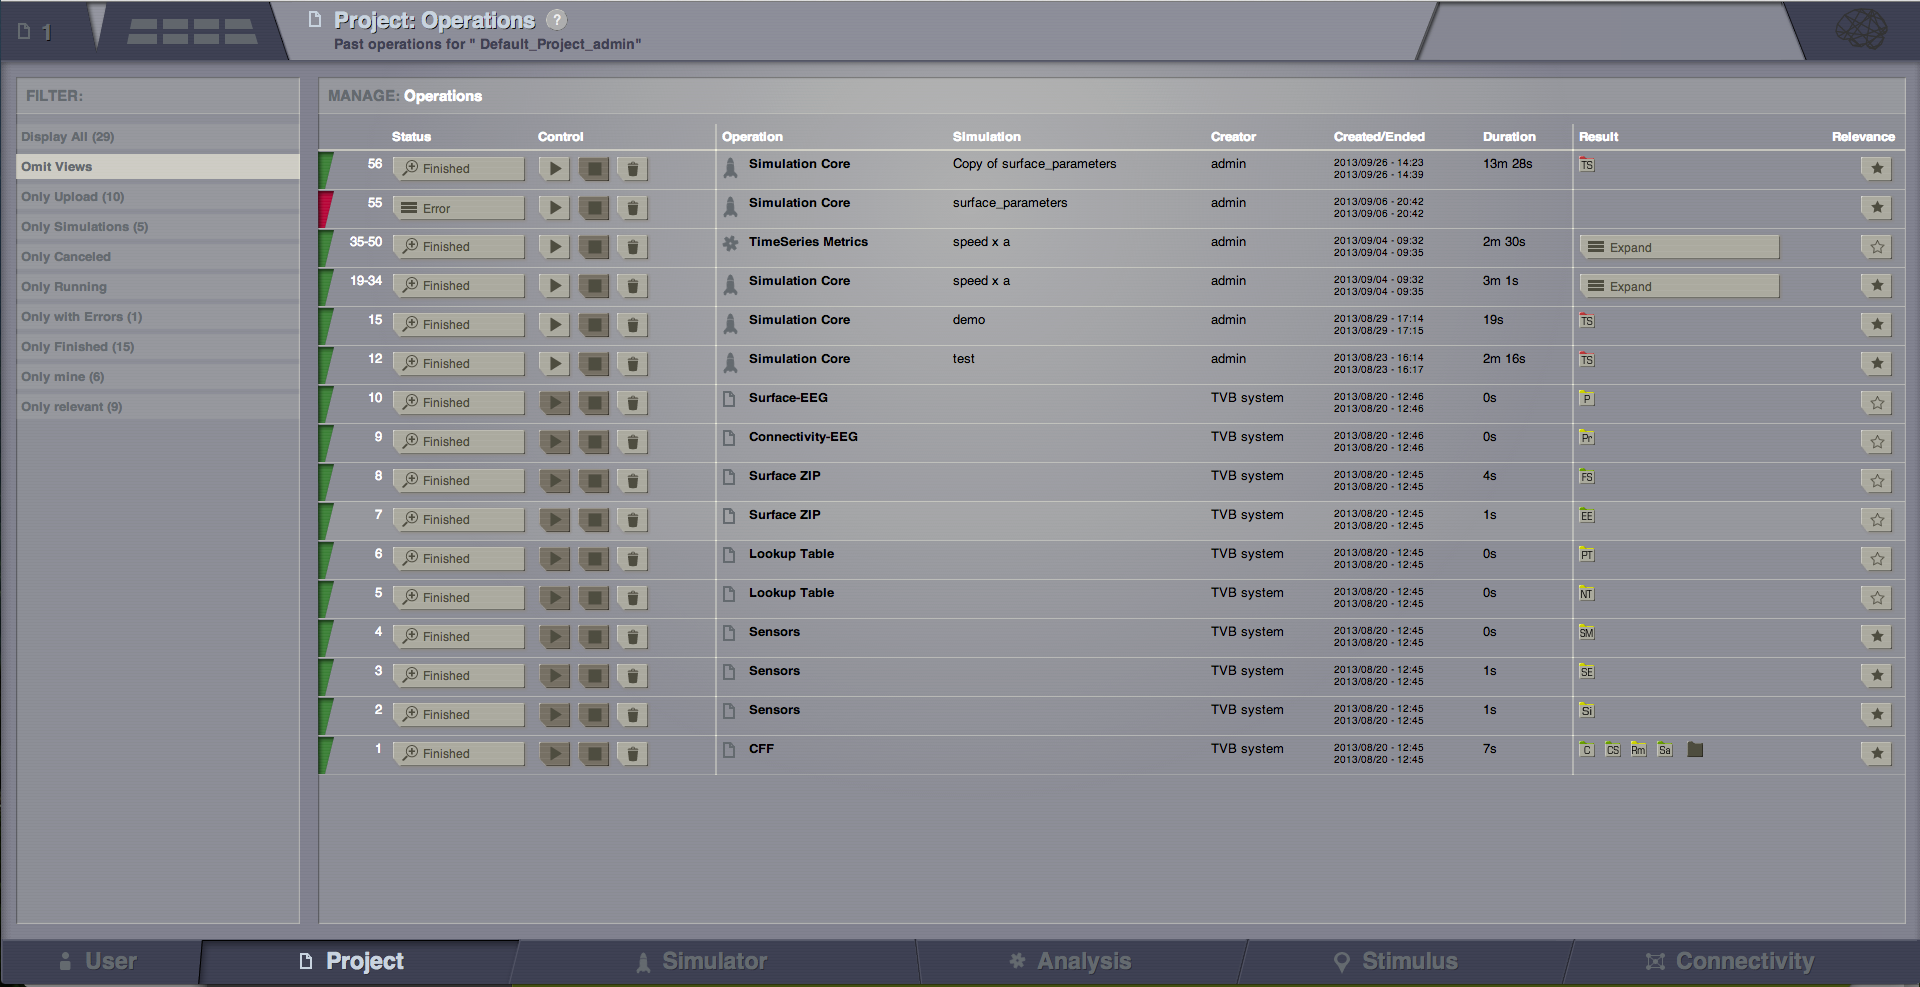
\includegraphics[width=0.47\textwidth]{images/ui_project_operations.png}}
		\\
		\subfloat[][]{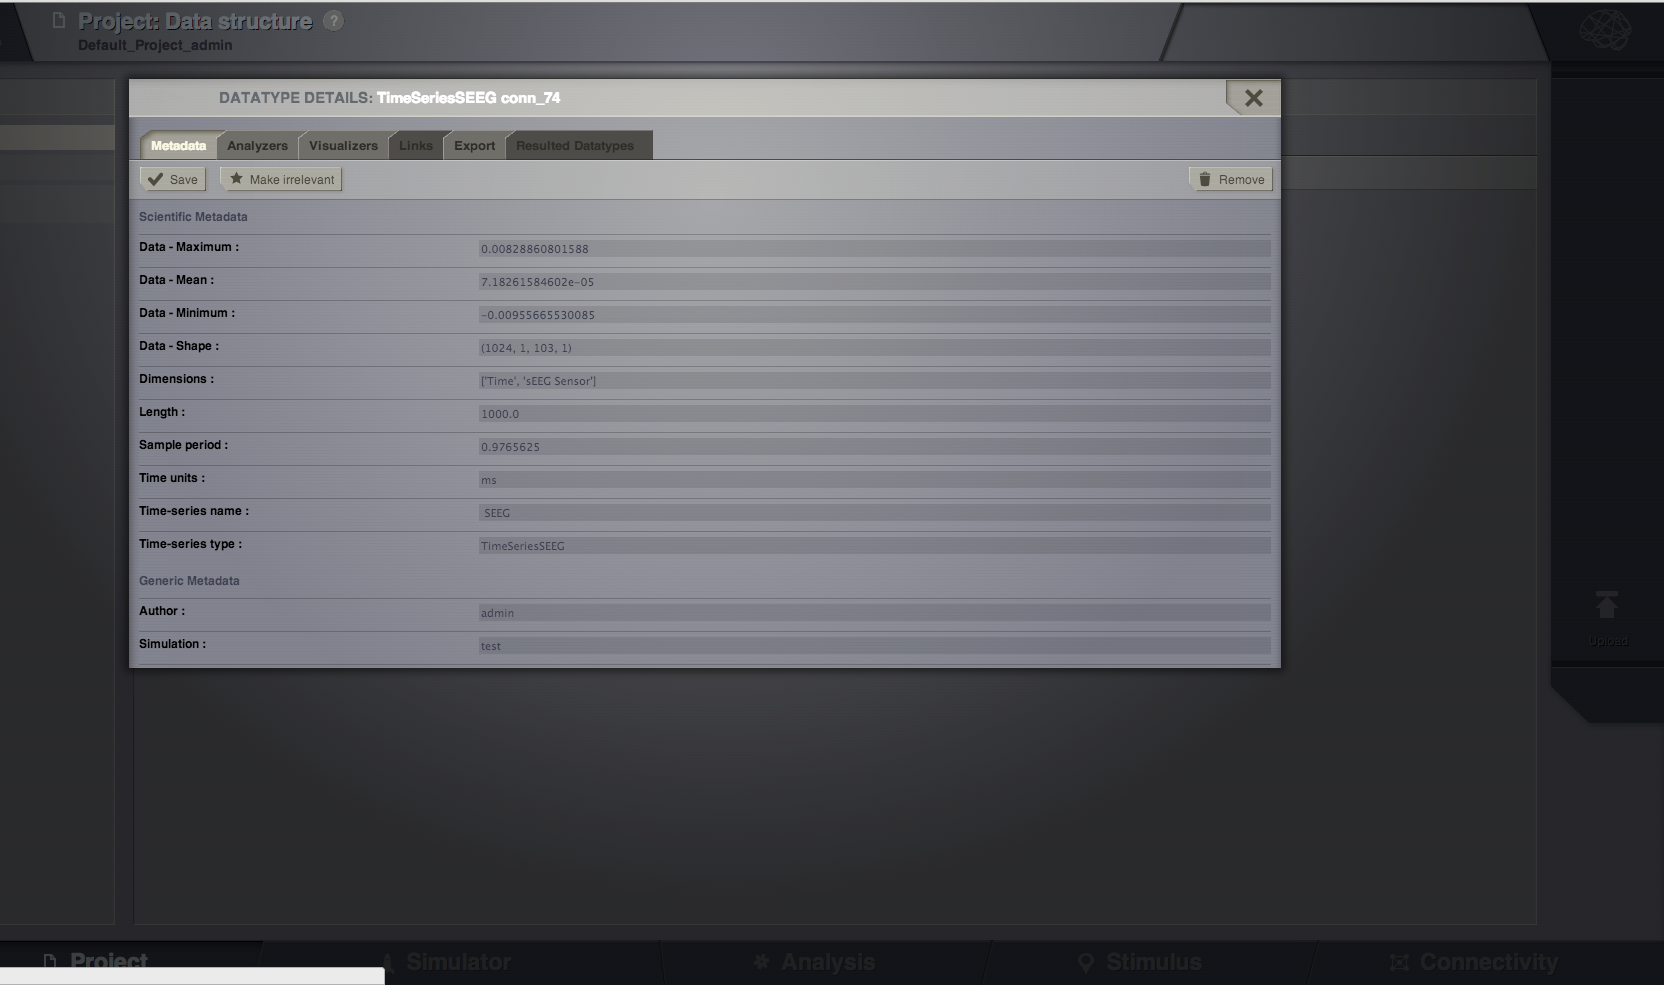
\includegraphics[width=0.47\textwidth]{images/ui_project_datatype_details.png}}
		\caption{\TVB Data Organization
		(A) View all Projects
		(B) 2D graph display of Operations with their input and output DataTypes 
		(C) View all Operations in current project with their status, duration, results, etc
		(D) DataType details and further available operations for it. This menu becomes available after clicking a DataType result from several places in \TVB }
				\label{fig:project}
\end{figure}

		An \emph{Account} or \emph{User} is needed for accessing \TVB through
		the web interface.  When \TVB web interface is fired for the first
		time, the G-User is requested to set his or her username and a
		password for the first account which acts under an
		\emph{administrator} role. Later on, more users can \emph{register}
		for other accounts, that should be previoulsy validated by the admin
		account.

		A \emph{Project} in \TVB is a logical grouping entity, which  can be
		used in several ways by the end-user;  for example one could choose to
		create a project for each experiment in \TVB, while others might
		create projects for each subject of a group. Each project has a single
		\emph{User} (or \emph{Account}) as owner, but a project can be shared
		with multiple users to allow for collaborative reasearch.

		Any execution of an Adapter results into an \emph{Operation} in the
		context of a project. Multiple operations will be executed under the
		same project. For example we will have operations created for each
		execution of a simulation, each run of a Fourier analyzer, or launch
		of a Brain Visualizer. An operation changes status over time, from
		\emph{started} into \emph{canceled}, \emph{finished successfully} or
		\emph{finished with error}. One operation can have multiple input and
		output parameters and parameters can be scalars or DataTypes.

		A \emph{Workflow} in \TVB is a set of operations with their artifacts,
		and wraps around a simulation as leading component. A workflow can be
		seen as a default \emph{tag} placed by the system on Operations and
		DataTypes  which are logically connected, as resulting one after the
		other. Custom tags can also be added by the end-user both on DataTypes
		and Operations, for tracking entities inside a Project.

		\subsubsection{Simulator Interface}

		The \emph{Simulator} page is a presented as configurable multicolumn interface that combines \TVB simulation, analysis and visualization functionalities (Fig.\ref{fig:simulator} A).

		\begin{figure}[!htbp]

		\centering
			\subfloat[][]{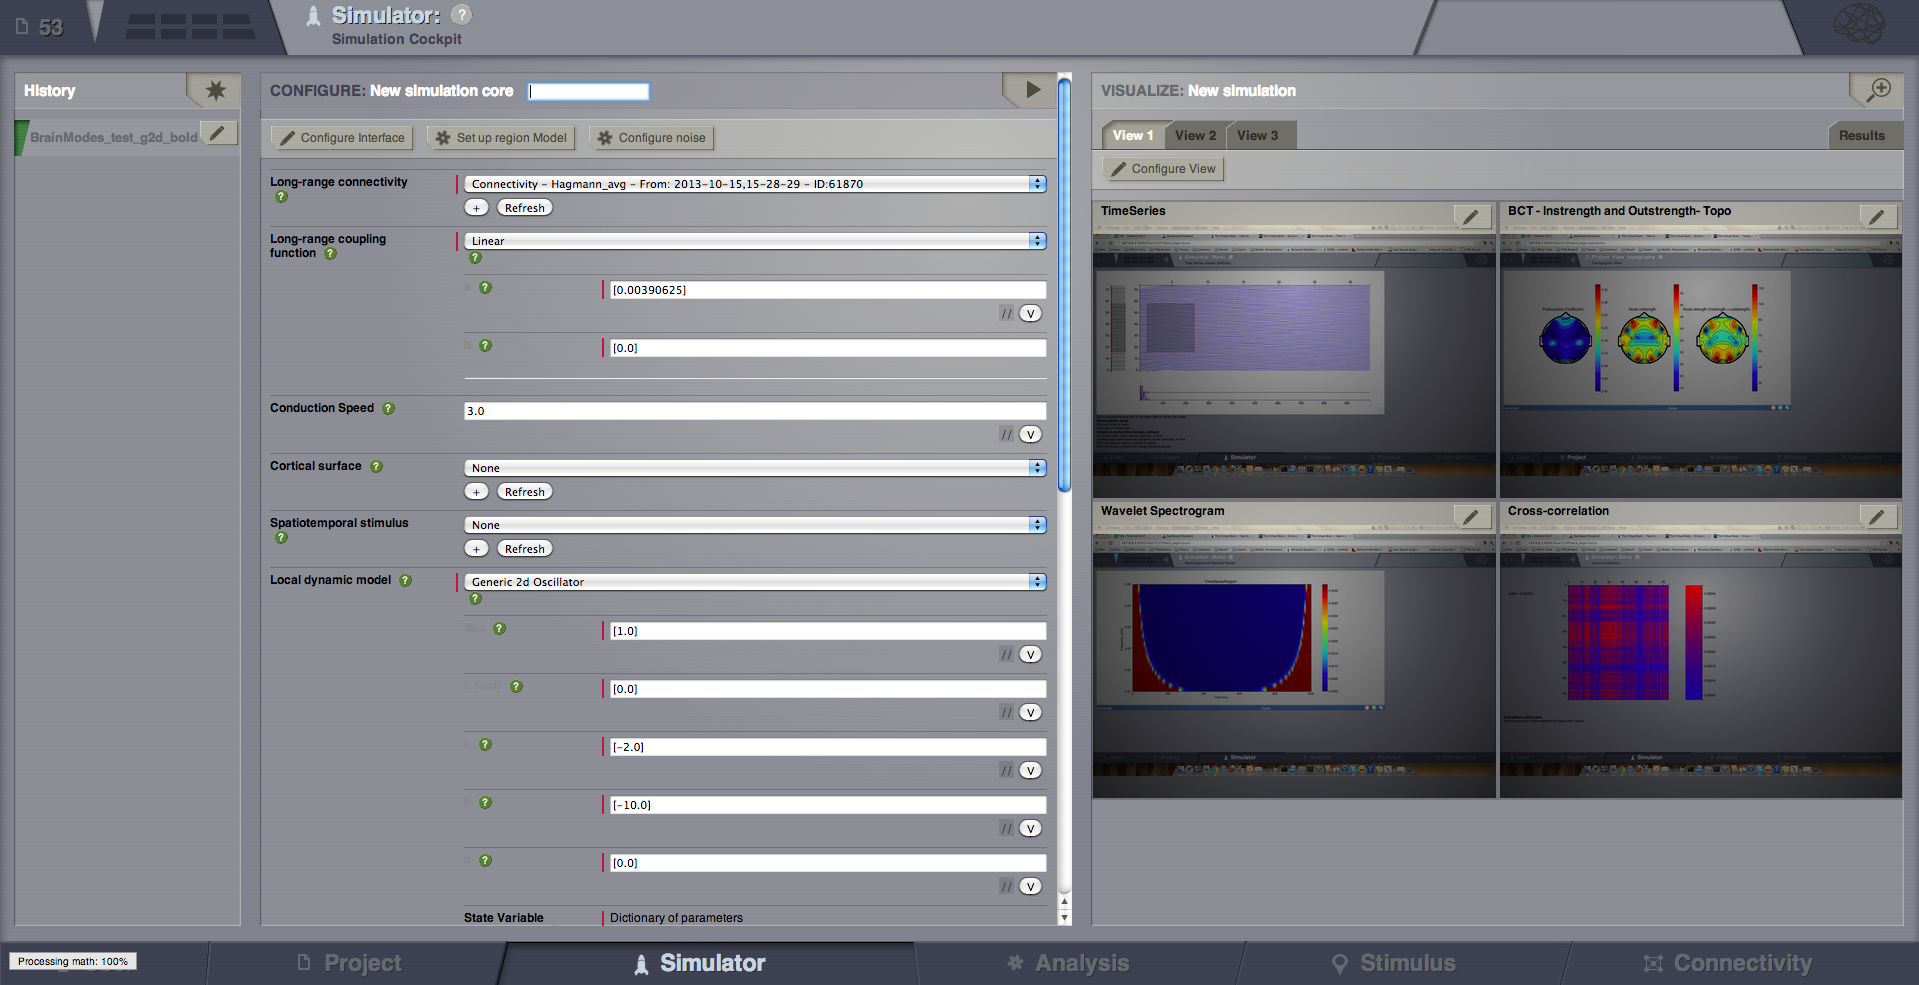
\includegraphics[width=0.47\textwidth]{images/ui_simulator.png}}
			\\
			\subfloat[][]{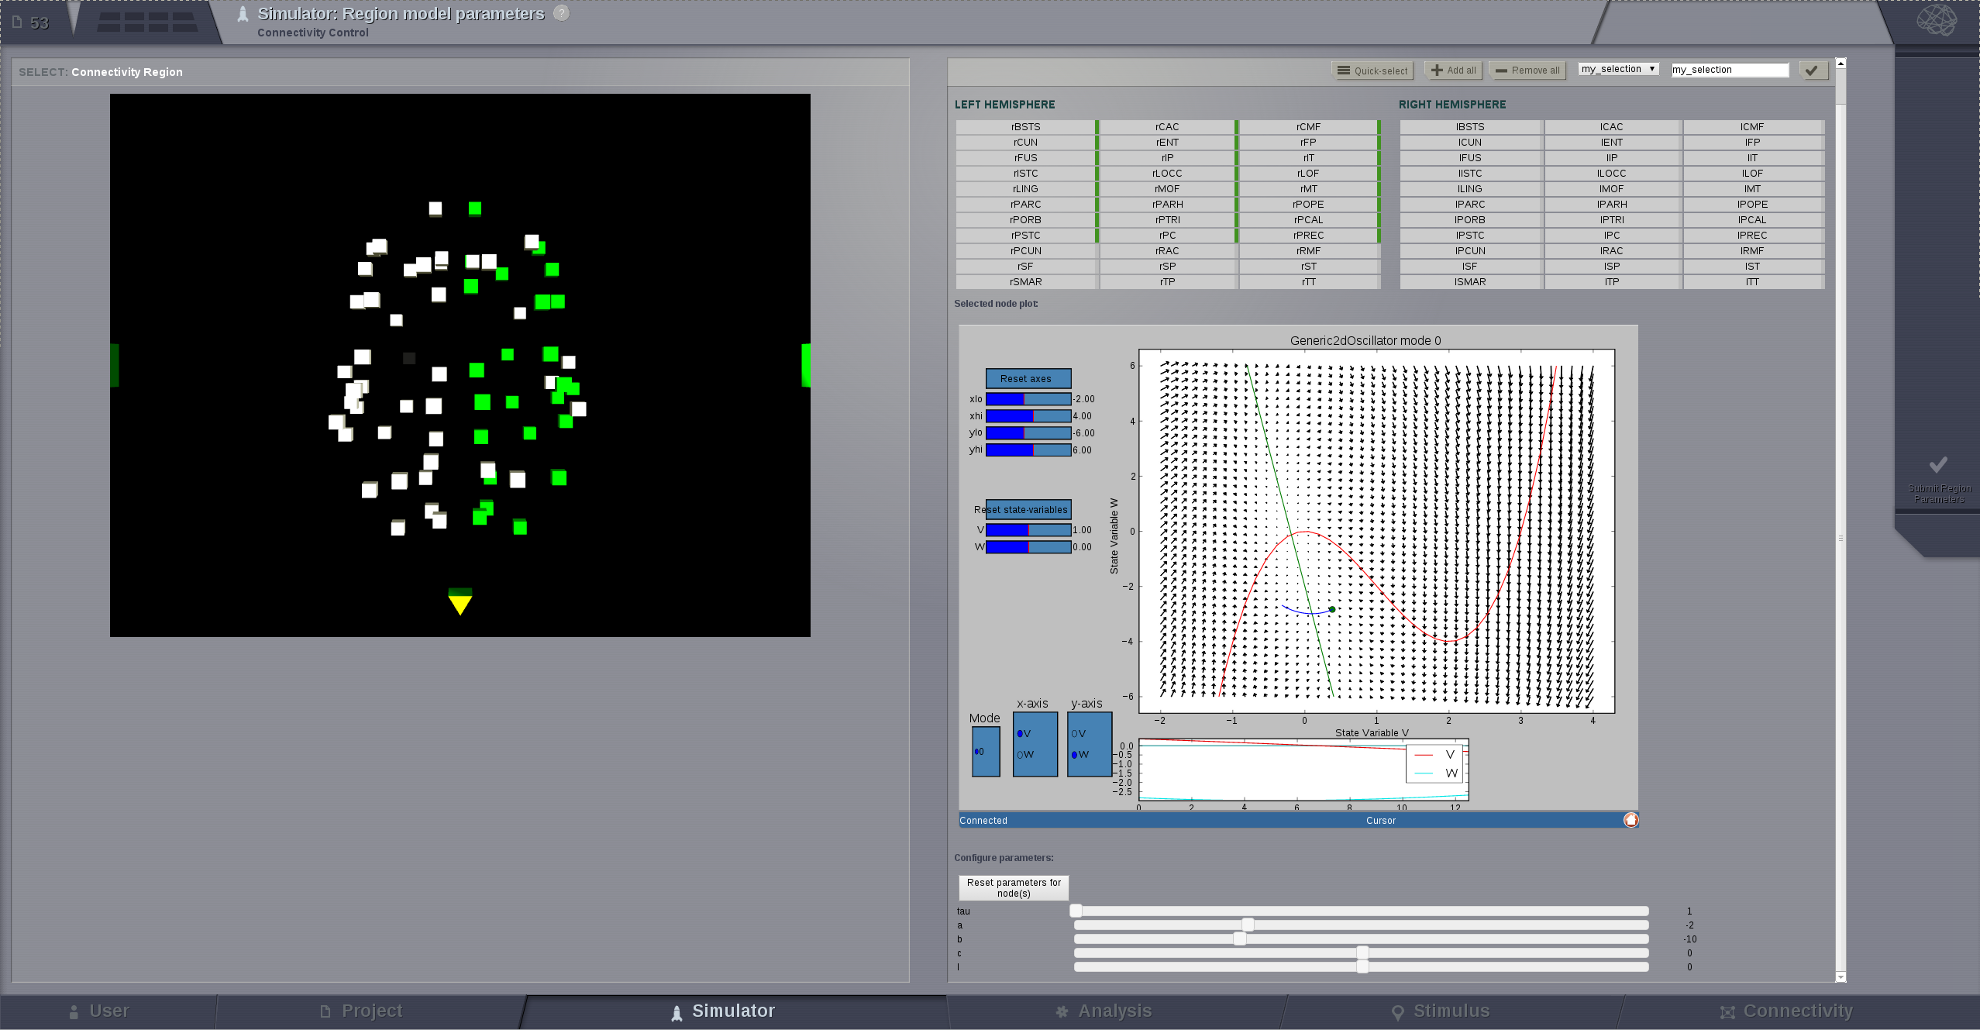
\includegraphics[width=0.47\textwidth]{images/ui_simulator_setup_region.png}}
			\\
			\subfloat[][]{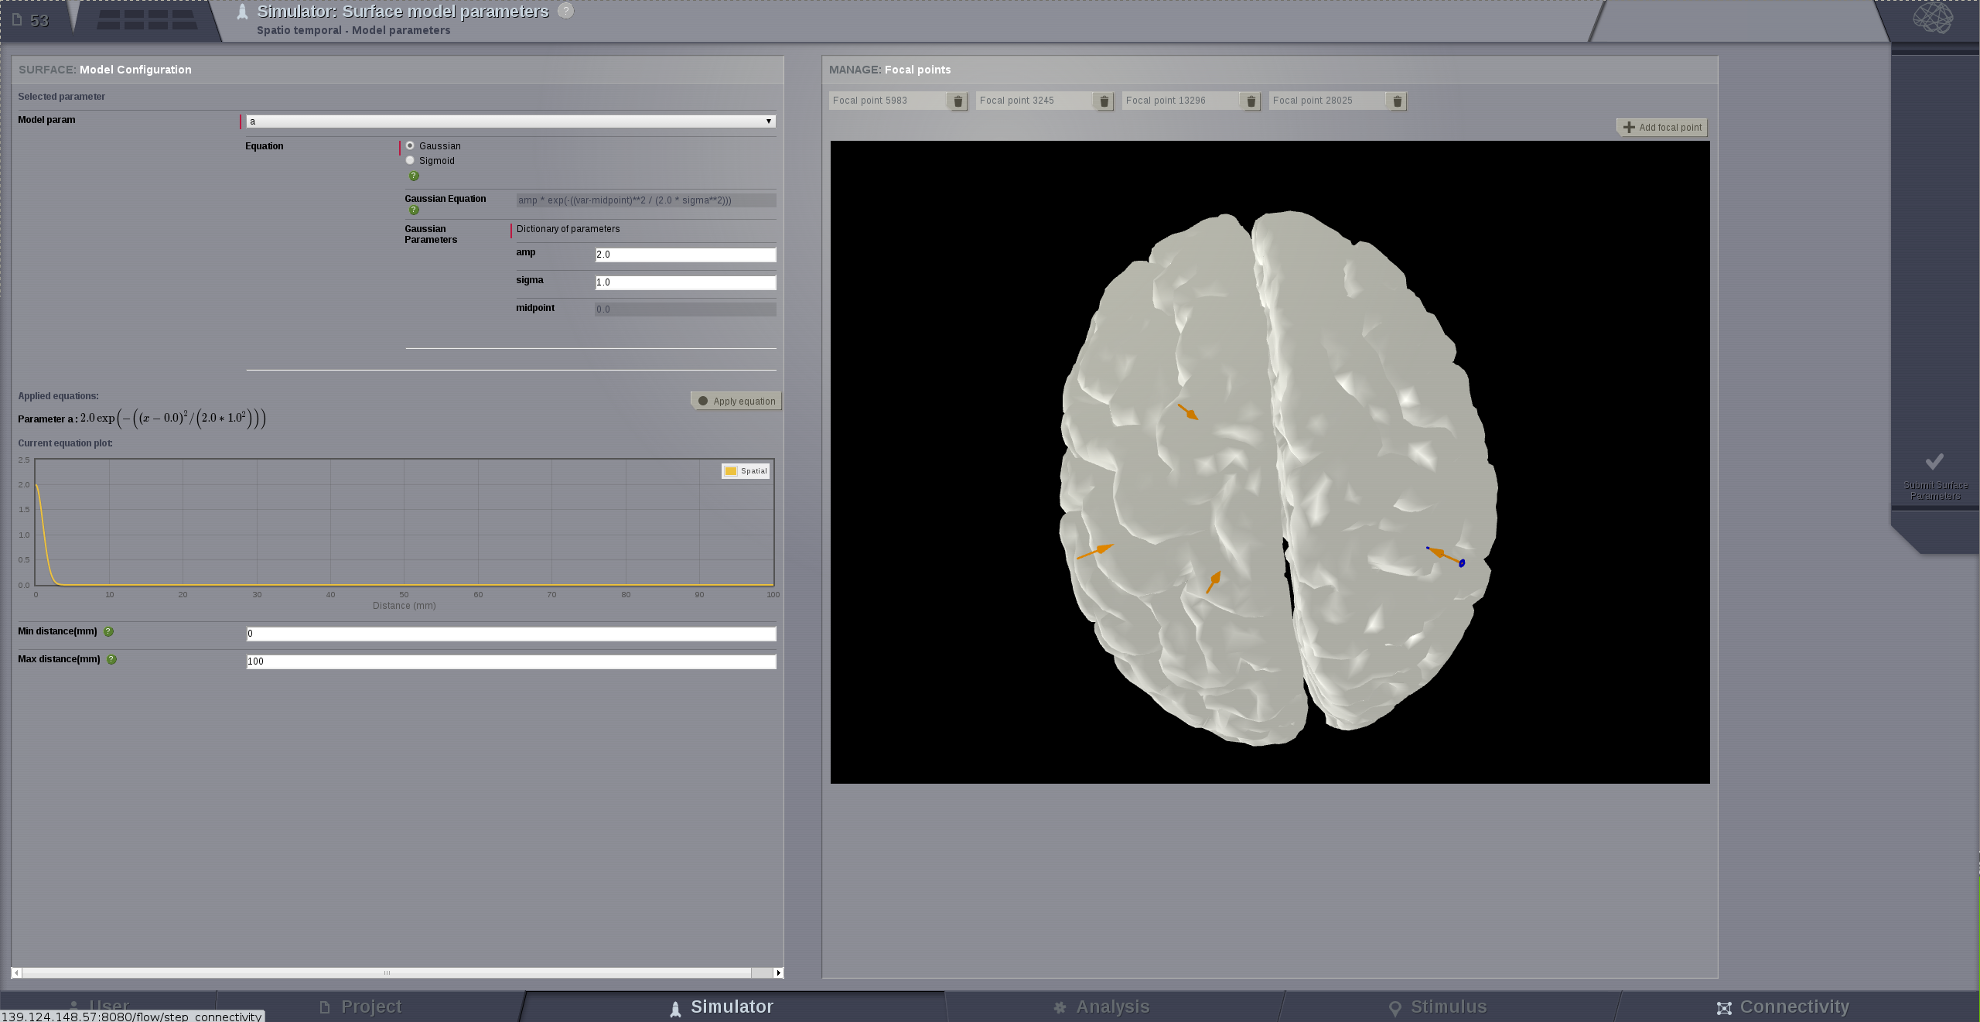
\includegraphics[width=0.47\textwidth]{images/ui_simulator_setup_surface.png}}
			\\
			\subfloat[][]{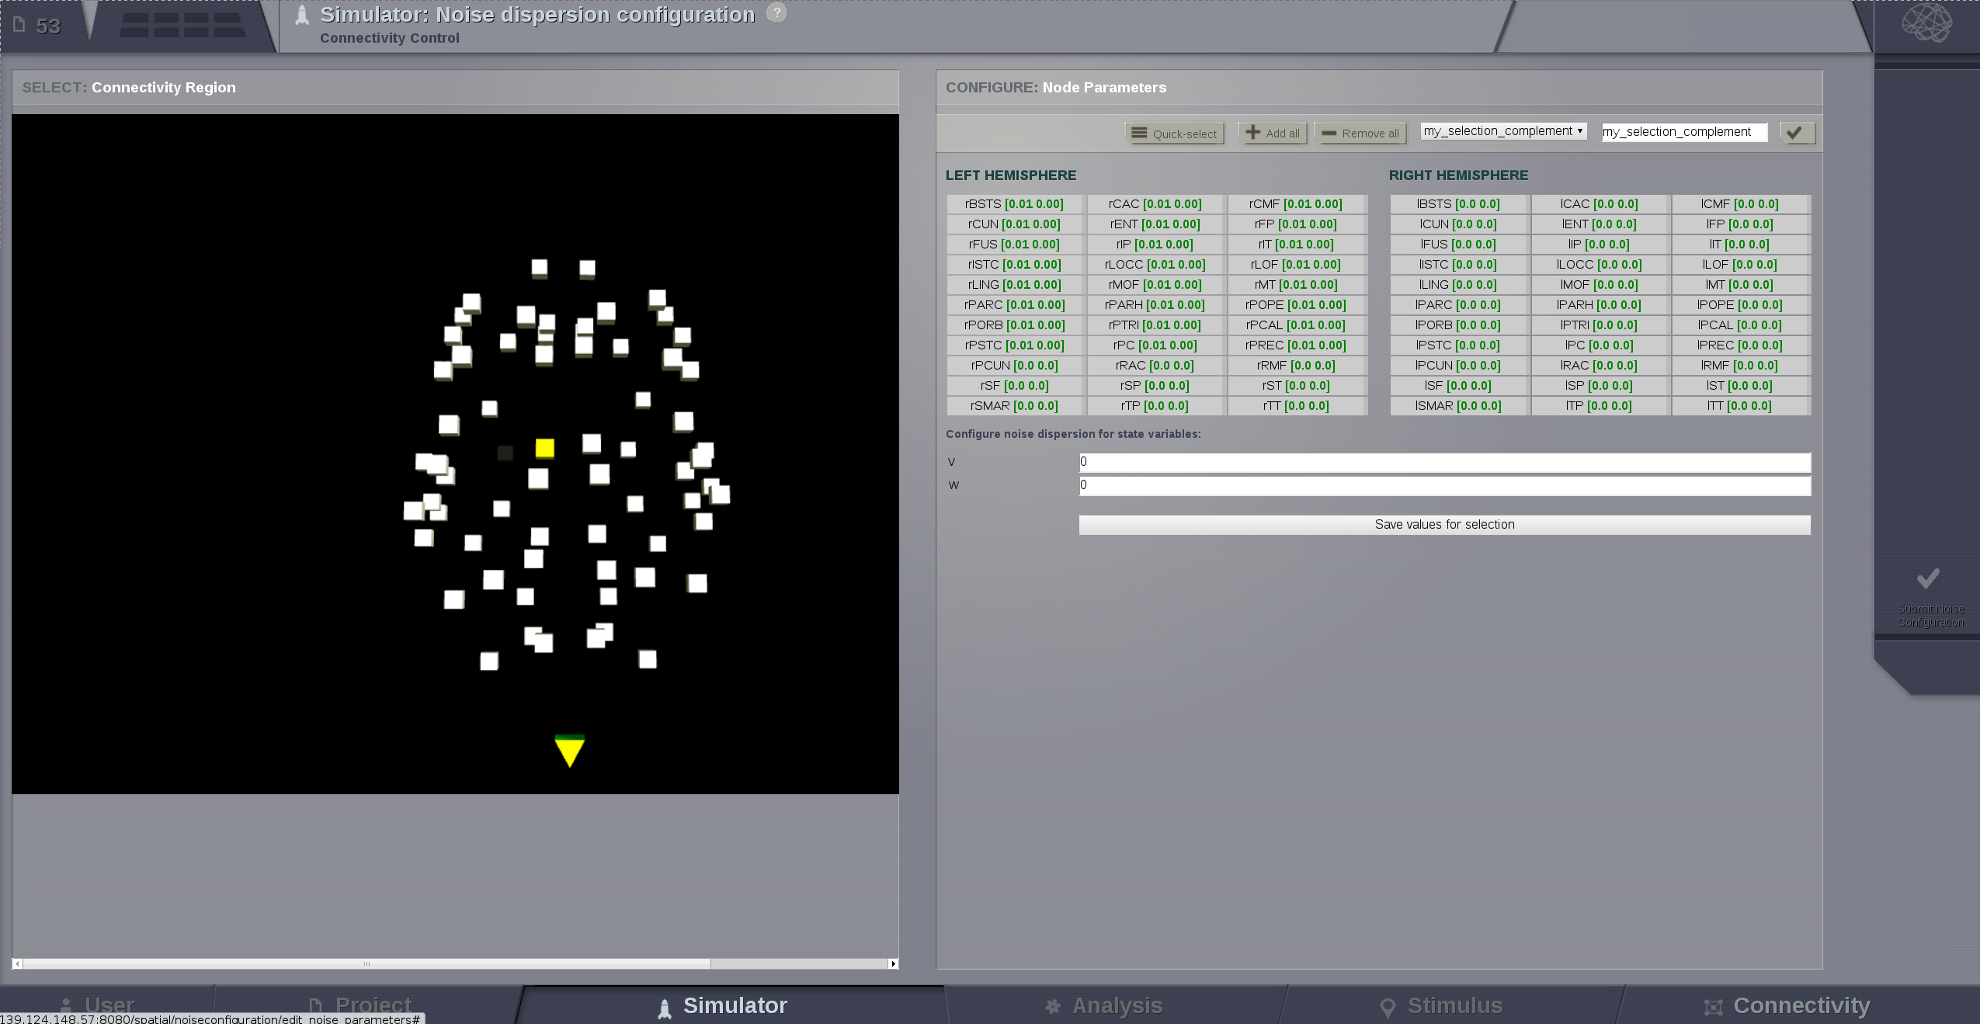
\includegraphics[width=0.47\textwidth]{images/ui_simulator_setup_region_noise.png}}
			\caption{\TVB Simulator Area: 
			(A) View of the main interface. Left, the history column keeps the information about the simulations and their status; middle, the simulation core column is where simulations are configured (e.g., change model, parameters, simulation length); and right, the visualization column, gives the possibility to configure visualizers to display the resulting time series or visualizers that will add an analysis step before displaying the results.  
			(B) Region-based simulation configuration area. The parameters of the local model can be set independently for each node, that is, the dynamics of each node may be different. 
			(C) Surface-based simulation configuration area. In a similar fashion, the model parameters are \emph{spatialized} by defining them as a function of a certain kernel (e.g., Gaussian kernel).
			(D) Noise configuration area. }
		\label{fig:simulator}
		\end{figure}

		On the left column, a history of all simulations is kept and can be 
		accessed at any time. Each simulation can be renamed or deleted.

		The middle column of the \emph{Simulator} area is where users configure their
		large-scale brain network model. On the top of this column there is a blank
		field to name each particular configuration and a button to launch simulations.
		Via this column, users have access to all the configurable components that might
		be used in a simulation, namely:

		{\small

		\begin{itemize}
			\item long range connectivity (i.e., the connectome or connectvity matrix);
			\item long range coupling function (to scale the weights in the connectivity matrix);
			\item conduction speed;
			\item cortical surface;
			\begin{itemize}
				\item local connectivity kernel;
				\item local connectivity strength (can be configured to be different for each vertex);
				\item region mapping (coorepsondances between vertices of the surface and anatomical reigons in the connectome);
			\end{itemize}
			\item stimulus
			\item local dynamics model (i.e. neural mass model)
				\begin{itemize}
					\item state variable range;
					\item state variables to be recorded and stored;
					\item initial conditions (seed and type of noise used to set random initial conditions);
				\end{itemize}
			\item integration scheme;
			\begin{itemize}
				\item if stochastic, the seed for numpy's rand can be set as well as the type of noise (white, coloured);
				\item integration time step size;
			\item monitors (you can set the monitors period to downsample the raw time-series)
			\item simulation length
			\end{itemize}
		\end{itemize}
		}

 \note[psl] Explain continuation feature.  

		Additional information about the components (e.g., modules, datatypes
		and their attruibutes) is available  by clicking on the interrogation
		mark icon next to each element. This documentation are pulled from the
		annotations from the traits system and doc strings.

		Specific pages are accesible for setting up the neural mass model
		parameters in region-based and surface-based simulations, as well as
		for configuring the noise amplitude in stochastic integrations (only
		for region-based simulations) (Figs. \ref{fig:simulator} B, C and D)
		The `Set up region Model` area consist of an interactive phase-plane
		display. This tool shows the 2-dimensional planes of the general
		n-dimensional phase space of the local dynamics model. This tool is
		used to observe how the dynamics of the physical model change as a
		function of its parameters.

		For surface-based simulations the model parameters are defined as
		function of distance from a central focal point (vertex of the
		surface). Thus, there is an extra layer of complexity by spatially
		varying the model parameters.

		On the right column, different displays can be configured to exhibit
		the simulated time series or to add an analysis step and see those
		results (e.g., compute the correlation coefficients and visualize the
		resulting matrix).

		It is possible to launch parallel simulations to systematically explore a set of
		components (e.g., a parameter of the  the local dynamics model, coupling
		strength, condution speed, among others. The resulting maps will be presented
		either in a discrete (Fig.\ref{fig:visualizers} A) or a continous 2D plot. 

		\note[psl]{Maybe mention that the value presented in the pse images is
		a float representing a certain charactersitic of a time-series
		collection (eg, for exploring synchronization one should use the
		kuramoto index parameter.)}

		
		\subsubsection{Analysis \& Visualizers}

			\TVB does not aim to compete at the analysis level with other tools in
			Neuroscience,  highly specialized and with great history in data
			analysis, like FSL \cite{Smith_2004, Woolrich_2009, Jenkinson_2012} ,
			SPM \cite{Friston_1995}, FieldTrip \cite{Oostenveld_2011} and
			Brainstorm \cite{Tadel_2011}.  What we offer is a minimalist set or
			algorithms to post-process your simulated results (or even process
			imported patient measured scans) inside \TVB, mainly for quick
			validations.

			We have created inside \TVB adapters for \emph{Fast ICA} from the
			python library \emph{sklearn},  we've implemented a python version of
			\emph{Fourier Spectral Analysis},  we have even wrapped the Matlab
			library \emph{BCT} \url{https://sites.google.com/site/bctnet/}, and
			others as analyzers.

			For each of the DataTypes produced in \TVB, one or multiple
			visualizers are available.   \TVB has couple of  visualizer types,
			each developed with the technology providing better support on the
			specific requirements for the visualization in course:

			 \begin{figure}[!htbp]
					\subfloat[][]{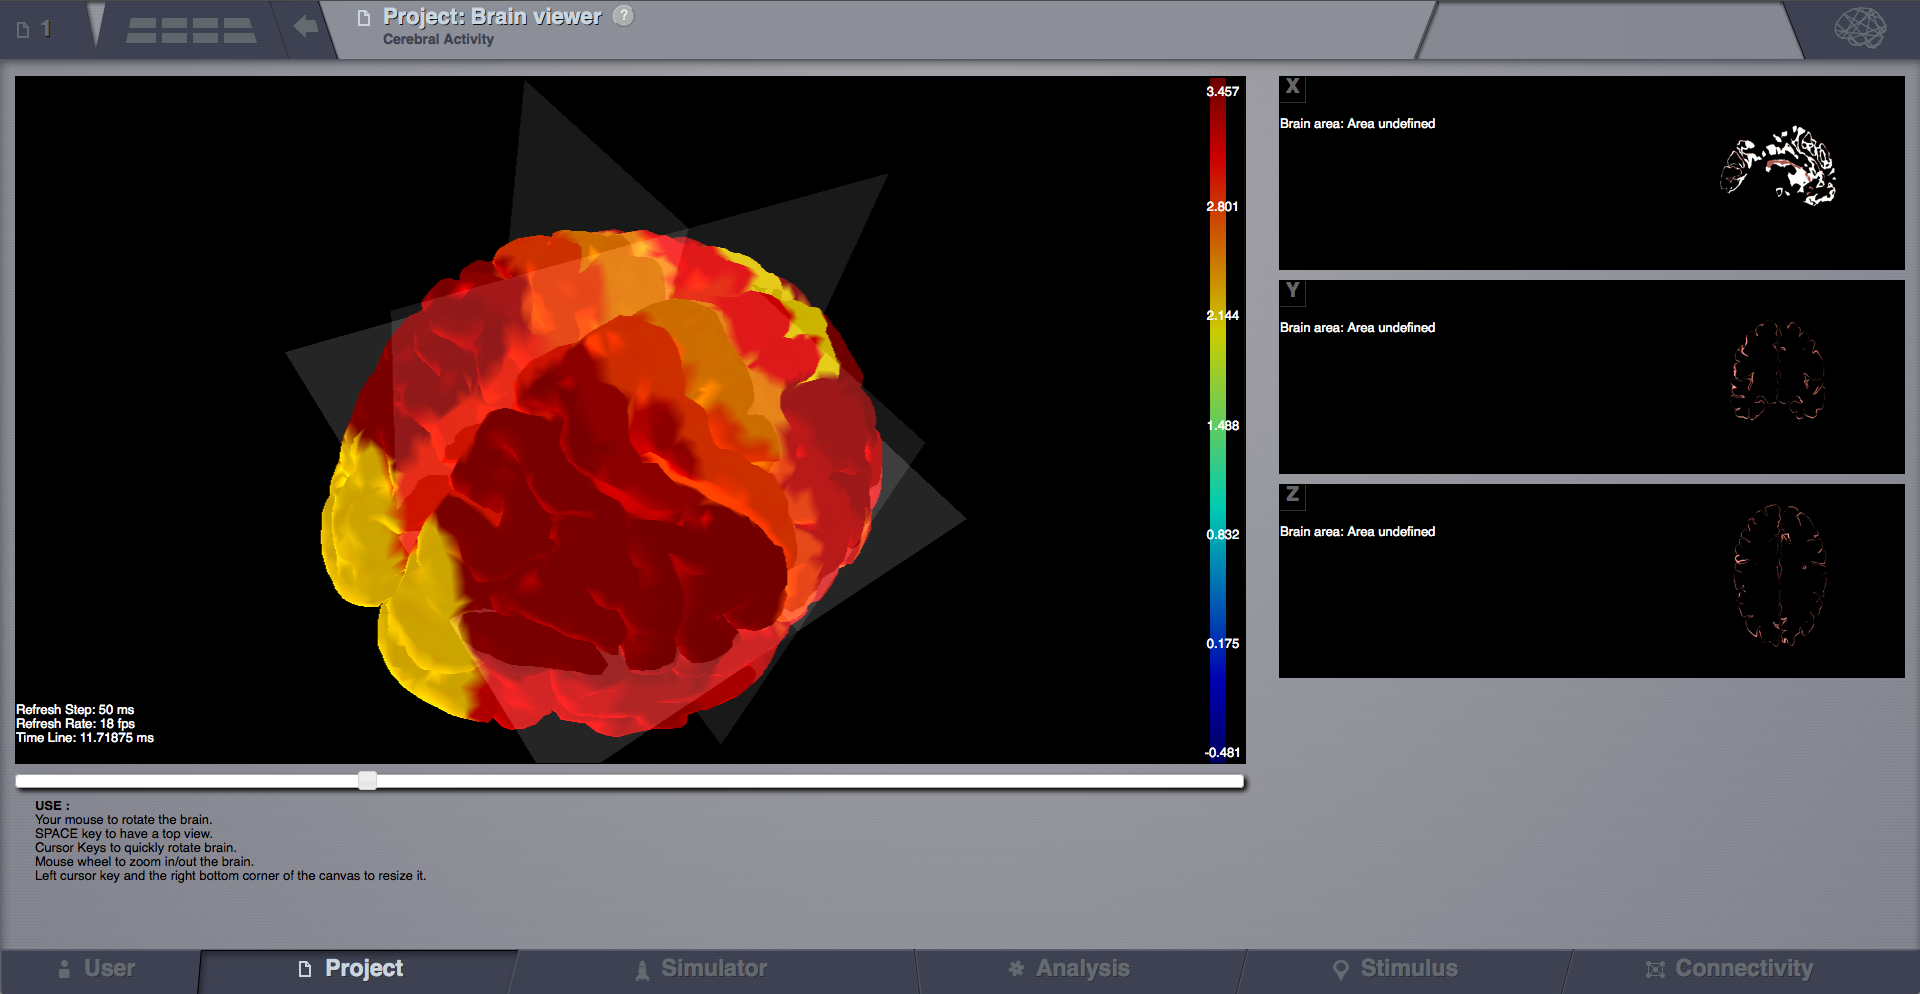
\includegraphics[width=0.48\textwidth]{images/ui_view_brain.png}}
					\\
					\subfloat[][]{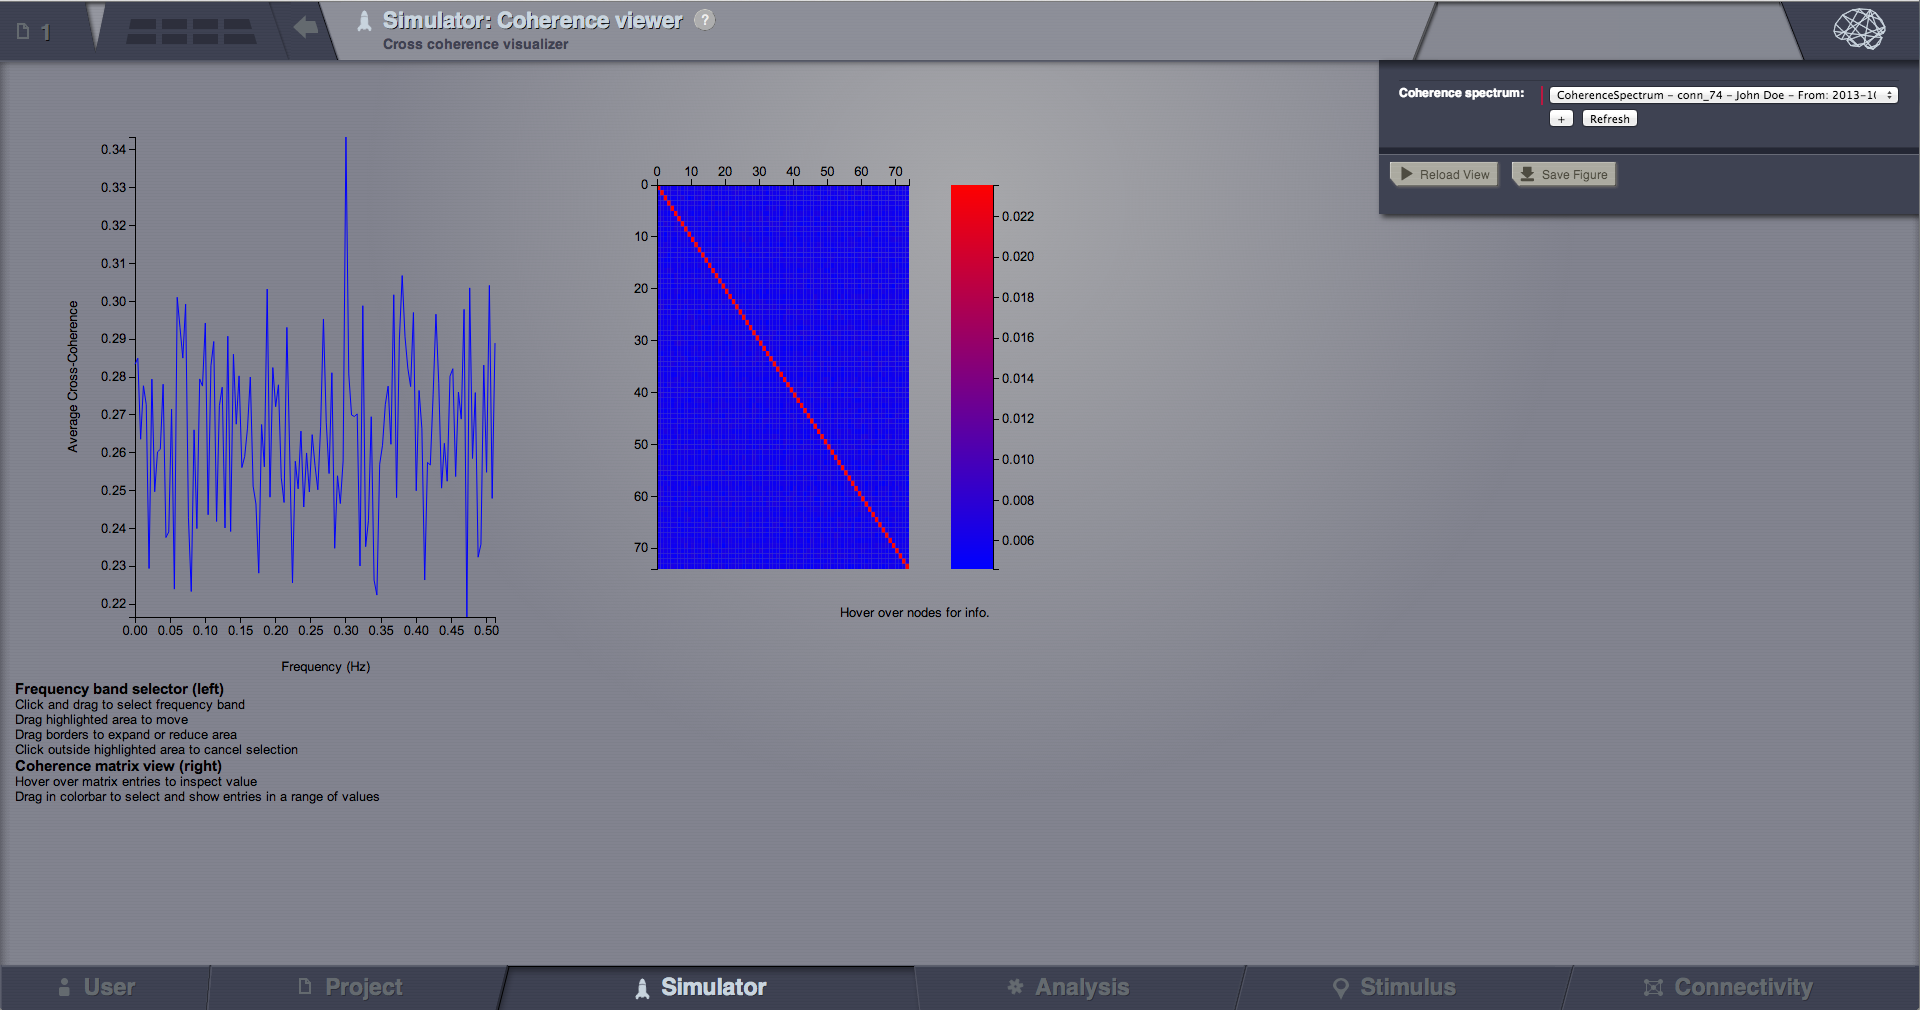
\includegraphics[width=0.48\textwidth]{images/ui_view_coherence.png}}
					\\
					\subfloat[][]{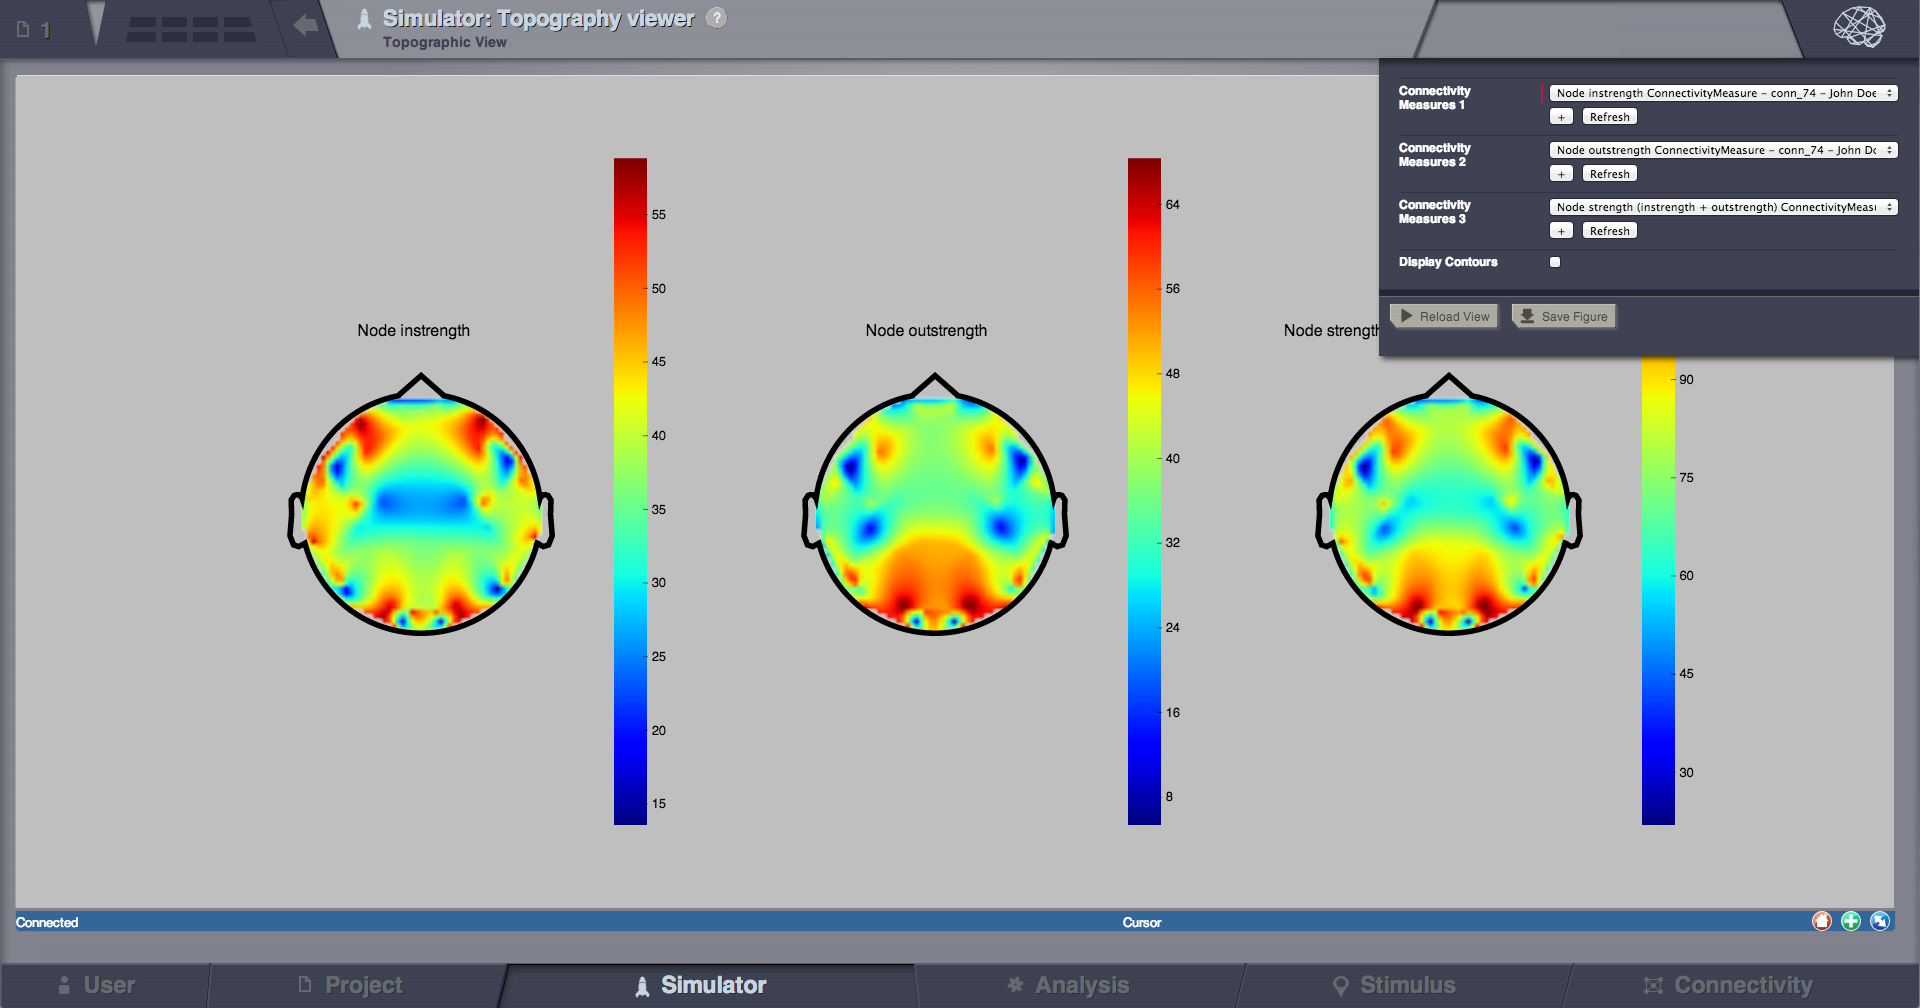
\includegraphics[width=0.48\textwidth]{images/ui_view_topo.png}}
					\\
					\subfloat[][]{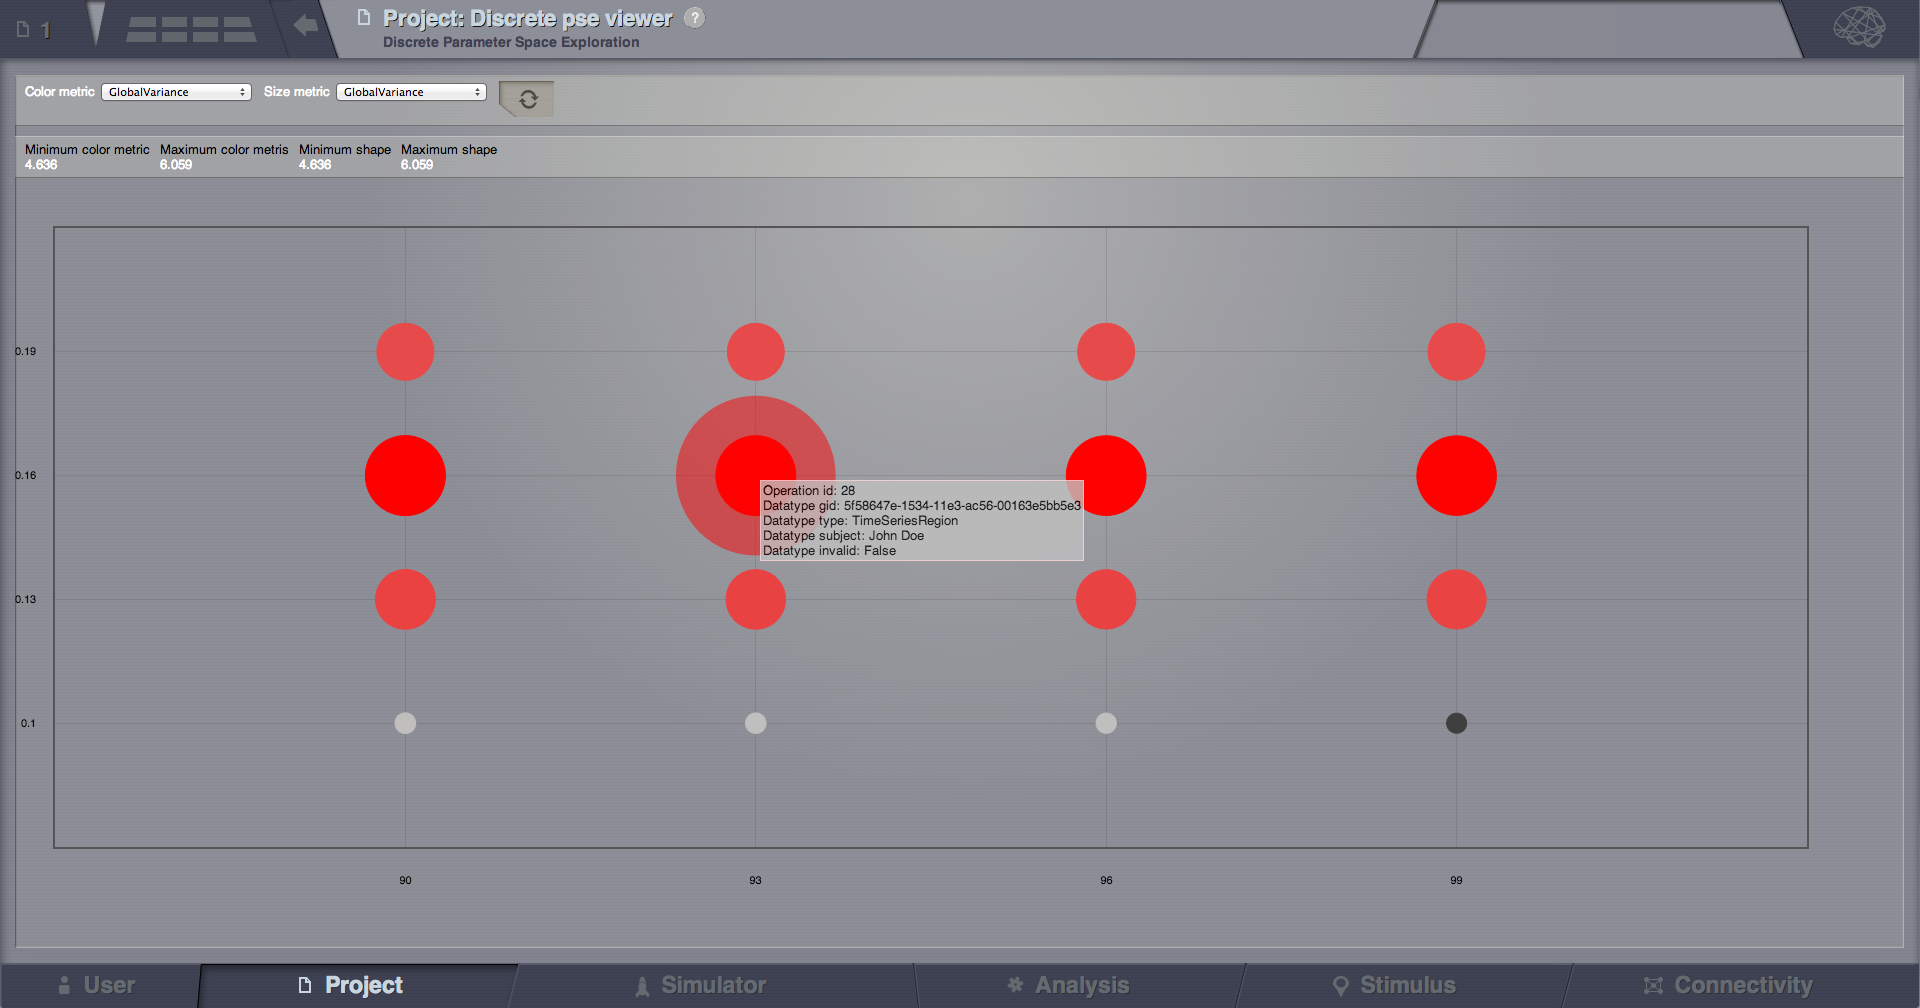
\includegraphics[width=0.48\textwidth]{images/ui_view_pse.png}}
					\caption{\TVB visualizers: 
					(A) WebGL: 3D display of region level simulated signal, mapped on a brain cortical surface
					(B) SVG: Cross Coherence
					(C) MPLH5:  Topograhic view with Connectivity in/out strength measures
					(D) FLOT: Parameter Space Exploration results grid}
				\label{fig:visualizers}
			\end{figure}
	
	\begin{enumerate}
		\item \emph{WebGL viewers:} are based on \emph{HTML 5 Canvas} element
		and the \emph{gl} context. These viewers offer 3D nice display,
		vectorial zoom support, user interaction with the scene (rotate,
		translate), quick response (even when thousands of vertices and edges
		are to be manipulated) and good resolution for the images exported.
		
		\item \emph{SVG viewers:} offer great selection, zoom and scaling
		effects and extraordinary quality for the exported artifacts, while
		having a relatively low number of elements to display on the page. We
		use such viewers for manipulating and displaying TimeSeries,
		Covariance or Cross Coherence DataType results. These visualizers
		were developed expressly for these data types in TVB, provided a 
		richer level of interaction that Canvas based visualizers.

		\item \emph{MPLH5 viewers:}  emph{Matplotlib} has an \emph{HTML 5}
		backend that we use for viewing some of \TVB DataTypes (like
		Fourier or Wavelet) url{https://code.google.com/p/mplh5canvas/}

		\item \emph{Other} simpler viewers in \TVB are using JIT
		\url{http://philogb.github.io/jit/} or FLOT
		\url{http://www.flotcharts.org/} - JS libraries. These are mainly
		2D graph displayers for some simple \TVB generated data.
	\end{enumerate}

\subsubsection{Connectivity Tools}

		\emph{Connectivity} in the context of \TVB is a DataType, mapping structural
		information about a subject (a real single individual or an average template). For
		editing and viewing a Connectivity, \TVB has a specific page, where
		the \emph{G-User} can manipulate connectivity strength and lengths
		starting from the granularity of an edge.

		We do not store or use information about the exact anatomical path or
		a connection, only the region centers and connection weights and
		lengths.

 \begin{figure}[!htbp]
		\centering
		\subfloat[][]{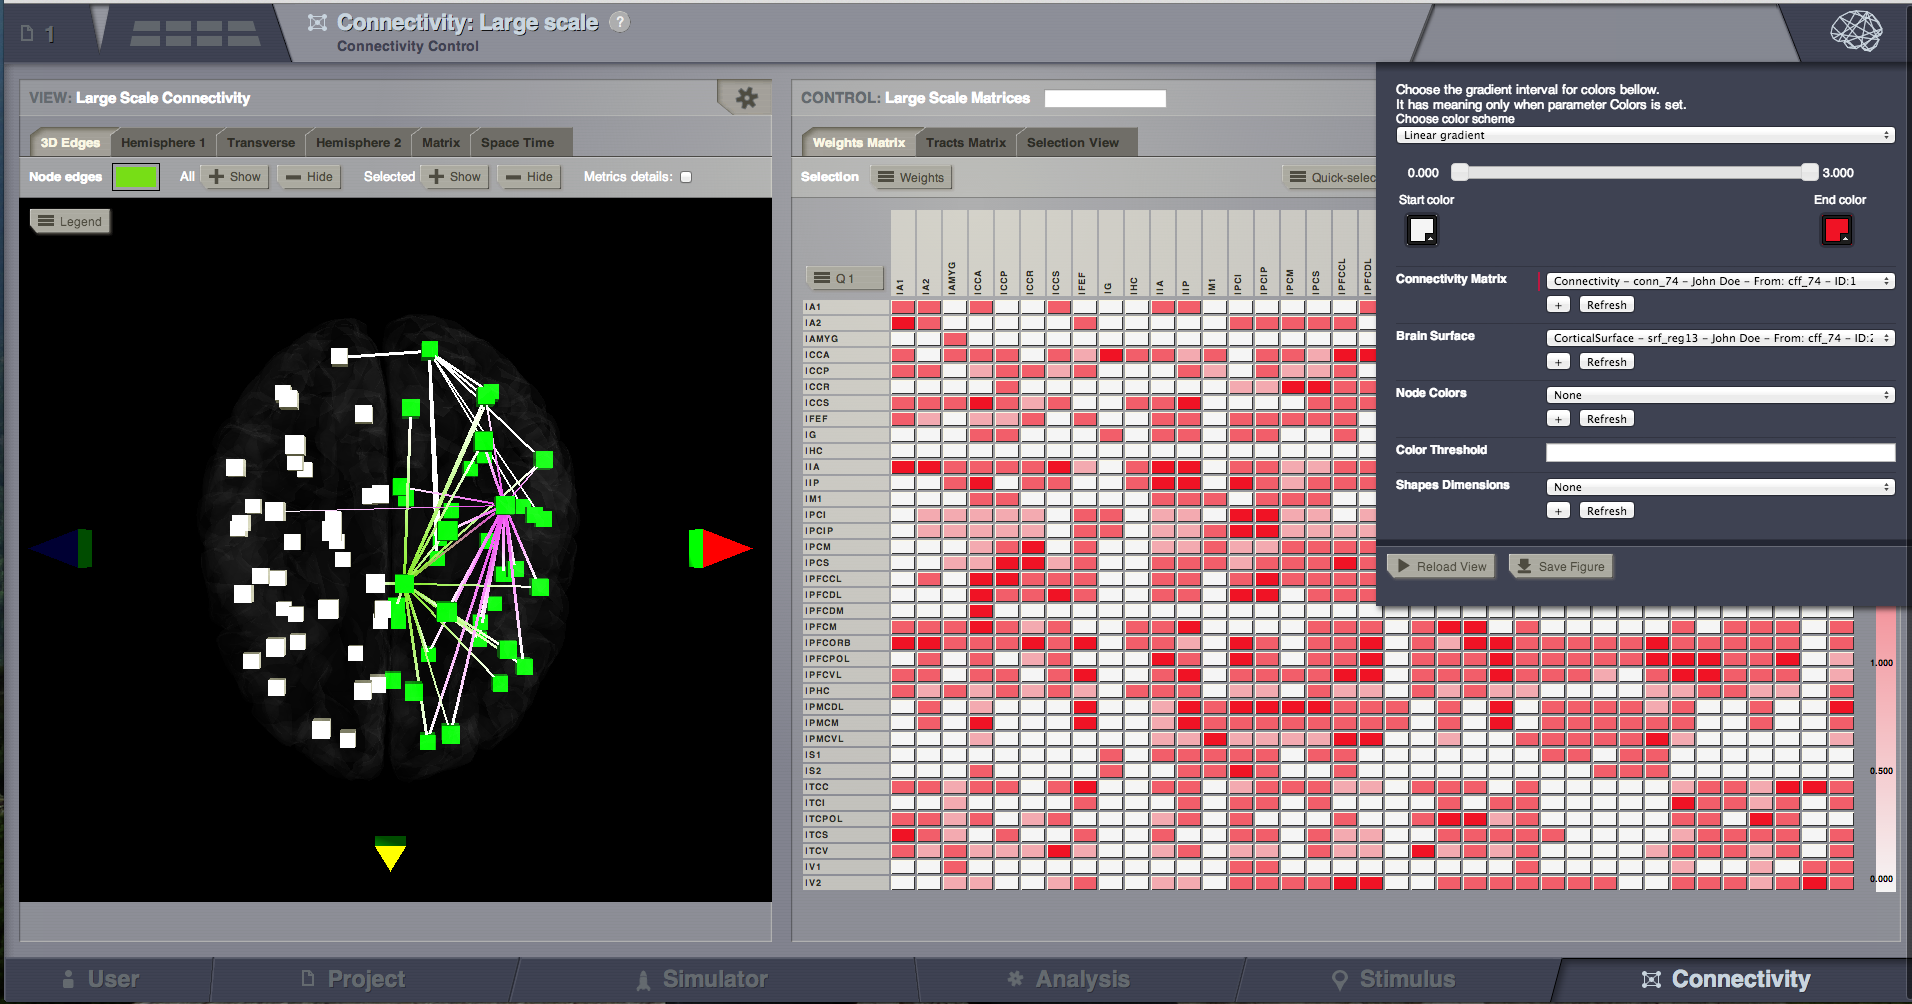
\includegraphics[width=0.48\textwidth]{images/ui_connectivity.png}}
		\\
		\subfloat[][]{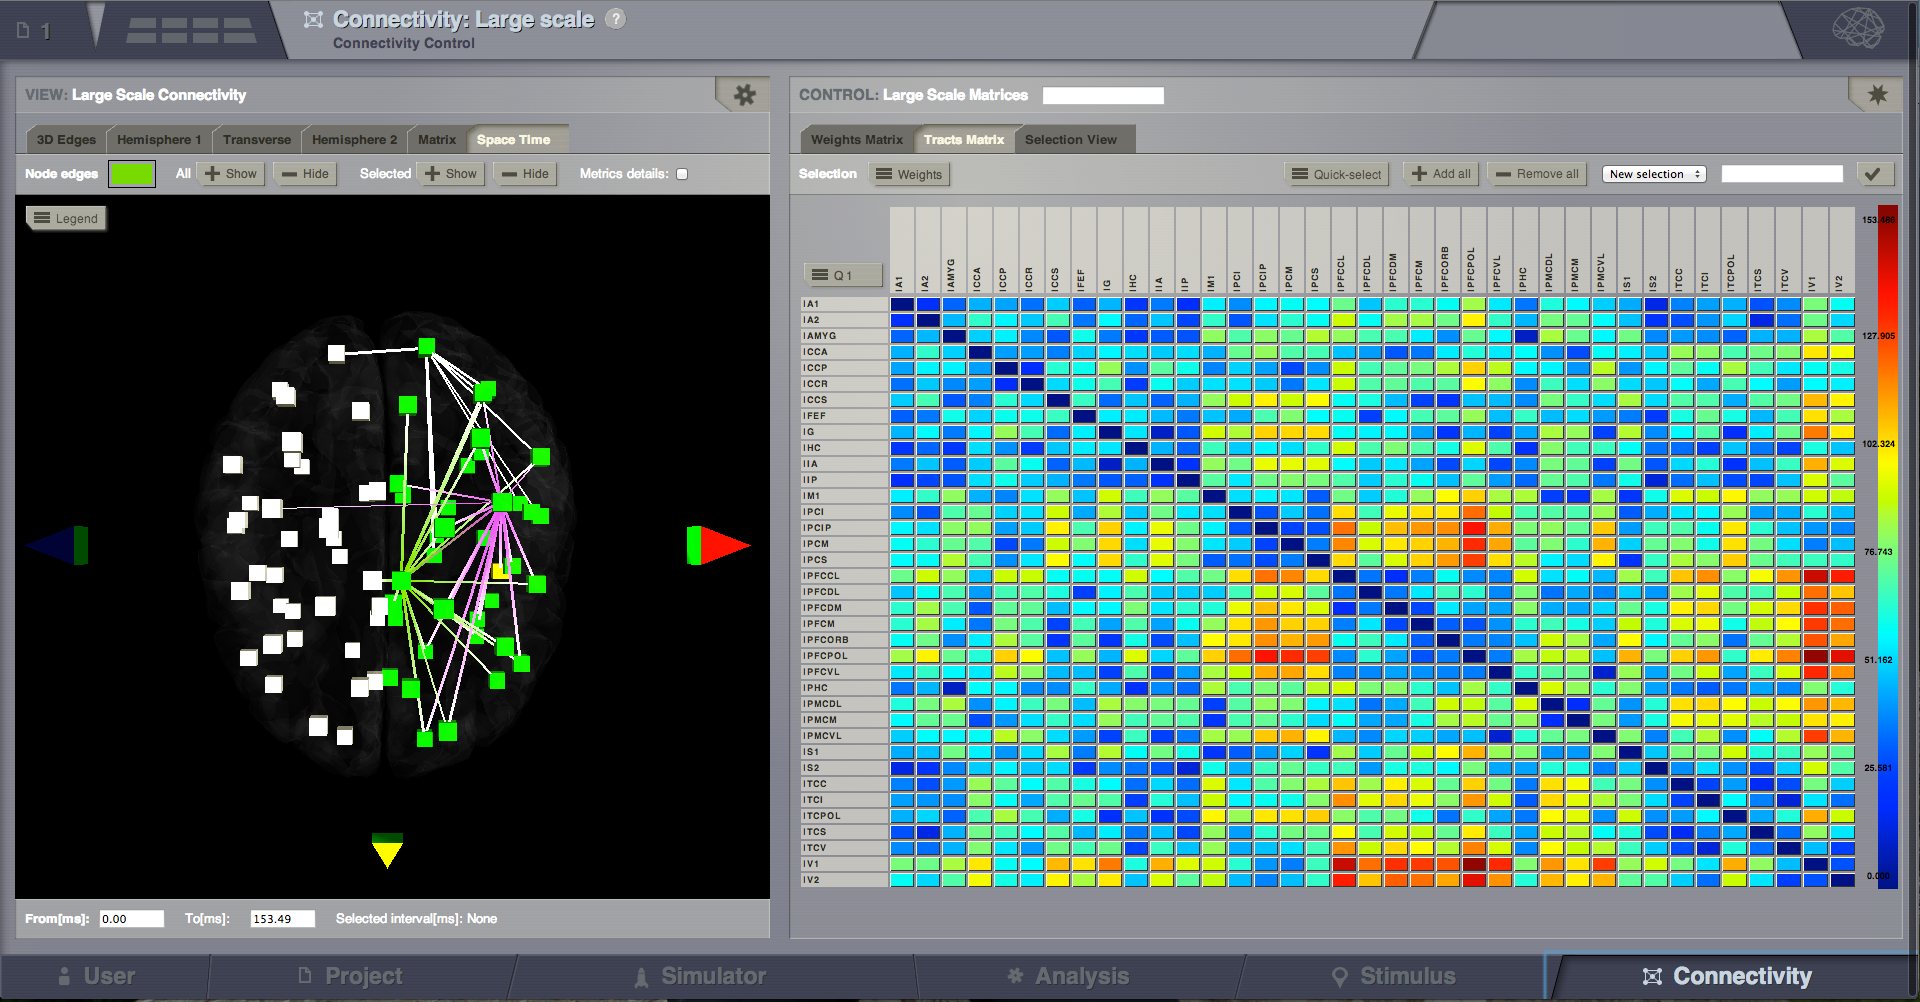
\includegraphics[width=0.48\textwidth]{images/ui_connectivity_delays.png}}
		\caption{Connectivity Tools: 
		(A) Left side: Displaying weighted connections between selection of nodes, with 3D manipulation.
		Right side: Editing weight connections, singular or bulk.
		(B) Left side: Show effect of connectivity delays (in milliseconds) when conductions speed is 1 mm/ms.
		Right side: Editing and displaying one quadrant from the matrix of connection tracts.}
				\label{fig:connectivity}
\end{figure}

\subsubsection{Stimulus Editor}

	In the \emph{Stimulus} area, an interactive environment assists users to
	generate stimulation patterns (e.g., a modeling study about TMS) that maybe be
	later included in a simulation.Similarly to the mechanism employed to vary
	model parameters from node to node, stimulation patterns are generated
	independently for region-based and surface-based simulations. In the former, a
	unique temporal profile can be specified for each node, although the amplitude
	of the stimulation can be modulated individually for each node. In the latter,
	in addition to the temporal profile, it is possible to select several vertices
	on the surface to define the foci around which a spatial pattern is centered
	(Fig. \ref{fig:stimulus}). A stimulation profile in \TVB is a Pattern
	datatype, and it can be either temporal or spatiotemporal depending the
	spatial support of the network.

	\begin{figure}[!htbp]
		\centering
		\subfloat[][]{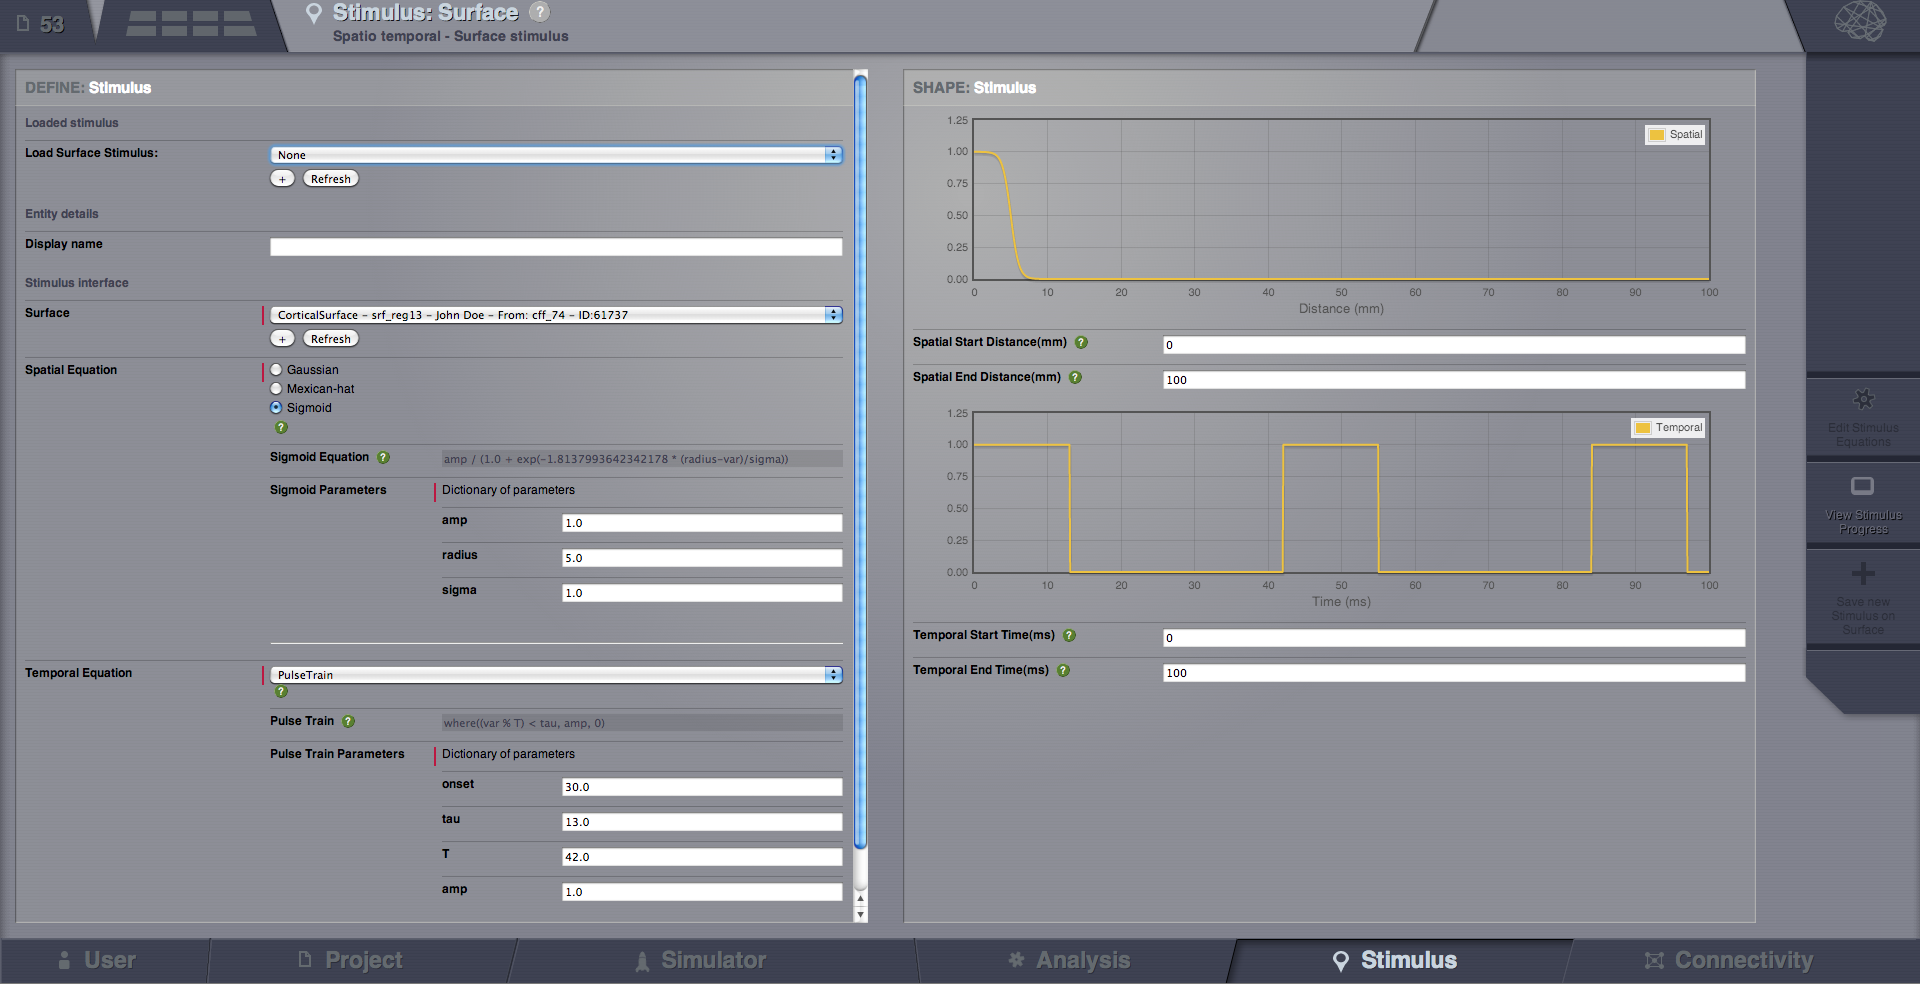
\includegraphics[width=0.48\textwidth]{images/ui_stimulus.png}}
		\caption{Stimulus Editor for a surface-based simulation.}
				\label{fig:stimulus}
	\end{figure}

	\note[psl] added the image for the sake of completeness, but maybe remove.  

\subsection{Console and scripting interface}

\note[lp]{How does it work?}

\subsubsection{Python Scripting}

The components of TVB are of course accessible from the a Python
script or, more conveniently, from any of the IPython interfaces.
For example, the tutorials for the simulator have been developed
as IPython notebooks, due to its ability to mix text, mathematics,
code and figures. 

\texttt{hello\_brain.py}
To give a basic feel for scripting TVB simulations, we will 
walk through a simple example of a region-level simulation shown in
Code~\ref{lst:uipython}

\lstinputlisting[caption={Python Listing},label={lst:uipython}]{python_lst.py}

%\begin{lstlisting}[caption={Python Listing},label={lst:py1}]
%from tvb.simulator.lab import *
%\end{lstlisting}

\noindent which is an all-in-one module making writing scripts
shorter, in the style of \texttt{pylab}, as it imports everything
from \texttt{pylab}, \texttt{numpy} and most of TVB's simulator
modules. Next, we build a simulator object:

%<<<<<<< HEAD
%\begin{lstlisting}
%sim = simulator.Simulator(
%		model        = models.Generic2dOscillator(), 
%		connectivity = connectivity.Connectivity(),
%		coupling     = coupling.Linear(a=1e-2),
%		integrator   = integrators.HeunDeterministic(),
%		monitors     = (
%				monitors.TemporalAverage(), 
%		)
%)
%\end{lstlisting}
%=======
%\begin{lstlisting}[caption={Python Listing},
%                   label={lst:py2}]
%sim = simulator.Simulator(
%    model        = models.Generic2dOscillator(), 
%    connectivity = connectivity.Connectivity(),
%    coupling     = coupling.Linear(a=1e-2),
%    integrator   = integrators.HeunDeterministic(),
%    monitors     = (
%        monitors.TemporalAverage(), 
%    )
%)
%\end{lstlisting}
%>>>>>>> lp

\noindent where we've employed a two dimensional oscillator
with default parameters, the default connectivity, a linear 
coupling function with a slope of $1e-2$, and deterministic
Heun integrator and a monitor that temporally averages the 
network dynamics before providing output.

While TVB strives to keep modules independent of one another,
it is typical for mathematical dependencies to arise between, 
for example, the mass model and the integration time step, so
after configuring a simulator object, it is necessary to invoke

%\begin{lstlisting}[caption={Python Listing},label={lst:py3}]
%sim.configure()
%\end{lstlisting}

which results in walking the tree of objects, checking and 
configuring the constraints among parameters recursively.

The next step is to run through the simulation, collecting
output from the simulator. In this case, it is as simple as
%<<<<<<< HEAD
%\begin{lstlisting}
%ys = array([y for ((t, y),) 
%					in  sim(simulation_length=3e2)])
%\end{lstlisting}
%=======
%\begin{lstlisting}[caption={Python Listing},label={lst:py4}]
%ys = array([y for ((t, y),) 
%	      in  sim(simulation_length=3e2)])
%\end{lstlisting}
%>>>>>>> lp

\noindent where the simulator has been called, returning a 
generator which performs the integration and returns, for each
monitor, the current time and activity. In a case where EEG 
and fMRI monitors, for example, were used, we might write
%<<<<<<< HEAD
%\begin{lstlisting}
%eeg, mri = [], []
%for (t_eeg, y_eeg), (t_mri, y_mri) in sim(3e2):
%		if y_eeg is not None:
%		eeg.append(y_eeg)
%		...
%\end{lstlisting}
%=======
%\begin{lstlisting}[caption={Python Listing},label={lst:py5}]
%eeg, mri = [], []
%for (t_eeg, y_eeg), (t_mri, y_mri) in sim(3e2):
%    if y_eeg is not None:
%	eeg.append(y_eeg)
%    ...
%\end{lstlisting}
%>>>>>>> lp

\noindent Because fMRI and EEG monitors have very different
timescales, whenever one monitor return data and the others do
not, the others contain \texttt{None}, hence the check. Building
more complex logic in this loop would permit, for example, online
feedback and modification of connectivity. 

After the simulation loop has finished, you may wish to see the
result, following the previous listing, 
%\begin{lstlisting}[caption={Python Listing},label={lst:py6}]
%plot(ys[:, 0, :, 0], 'k', alpha=0.1)
%\end{lstlisting}
\noindent Here we note that \texttt{ys} is four dimensional. The 
simulator has the convention of treating  mass model state as a
three dimensional array of state variables by nodes by statistical
modes. Because \texttt{ys} is an array collected over time, the first
dimension is time, and the plot here is of each node's first state
variable, over time.

Many more demonstrations of the various features of the simulator
can been found in scripts distributed with the sources of TVB, or 
browsed online at \url{https://github.com/the-virtual-brain/scientific_library/tree/trunk/tvb/simulator/demos}.

For more details see the Ipython notebook Tutorial: Anatomy of a Region Simulation 
\url{http://nbviewer.ipython.org/urls/raw.github.com/the-virtual-brain
/scientific_library/trunk/tvb/simulator/doc/tutorials/Tutorial_Anatomy
_Of_A_Region_Simulation/Tutorial_Anatomy_Of_A_Region_Simulation.ipynb}

\subsection{MATLAB Scripting}


\subsection{MATLAB Scripting}

Due to the popularity of MATLAB in the neuroscience community, an
interface from MATLAB to \TVB has been introduced that allows a MATLAB
script to design a TVB simulation, run it on TVB and retrieve the 
results. The MATLAB toolbox is provided separately from TVB, at
\url{https://github.com/the-virtual-brain/matlab-tvb}.
In the following, we give a short demonstration and 
describe implementation and rationale.

Because the MATLAB functions need to know the address of the server,
so we take any of the URLs used by the Web UI (here, the one provided
when launching TVB):

\begin{lstlisting}
sv = vb_url('http://127.0.0.1:8080/user/')
\end{lstlisting}

To run simulations without blocking MATLAB, a multiprocessing Pool
is used. We reset the pool and change the number of processes to 6

\begin{lstlisting}
vb_reset(sv, 6)
\end{lstlisting}

Next, we can query the server for information on the classes available,
and also get help for each of the classes

\begin{lstlisting}
info = vb_dir(sv);
\end{lstlisting}

\noindent where info is a cell array of structs, one per module (models,
monitors, etc.) and each struct has a field per class (models.JansenRit, 
models.Kuramoto, etc.). Each of these fields contains the details on 
the class, including all the parameters that can be set. 

To build a simulation, we start with an empty struct
and fill in the details for each part

\begin{lstlisting}
sim = [];

sim.tf = 1e3 % simulation length milliseconds
sim.model.class = vb.models.Generic2dOscillator;
sim.model.a = -2.1;

sim.connectivity.class = 'Connectivity';
sim.connectivity.speed = 4.0;

sim.coupling.class = 'Linear';
sim.coupling.a = 0.002;

sim.integrator.class = 'HeunDeterministic';
sim.integrator.dt = 1e-2;
\end{lstlisting}

Monitors are specified similarly but as a cell array there may be
several of them:

\begin{lstlisting}
sim.monitors{1}.class = 'TemporalAverage';

sim.monitors{2}.class = 'Raw';
sim.monitors{2}.period = 1.0; % ms
\end{lstlisting}

\note[sk]{Raw monitor has no period, or rather the period can't be set as it is
fixed as the integration time step...}

Lastly, we submit the struct as a new simulation

\begin{lstlisting}
[id, data] = vb_new(sv, sim);
\end{lstlisting}

\noindent Lastly, results are returned in a struct, here named data
where each field contians the output of a monitor and can be plotted
and analyzed as a regular MATLAB dataset:

\begin{lstlisting}
plot(data.mon_0_TemporalAverage.ts,...
     squeeze(data.mon_0_TemporalAverage.ys)')
\end{lstlisting}

The implementation of this interface is a combination of an additional
CherryPy controller providing an HTTP/JSON API, running on the same 
server as the Web UI, and a set of MATLAB functions that send HTTP 
GET requests to the server. An implementation based on MEX functions 
invoking the Python library directly was considered, for reasons of 
performance, however, it was judged that such an implementation may be
difficult to stabilize and maintain, given that it would require binary
compatibility between MATLAB, Python and the C compiler. Two additional 
advantages of an HTTP API are that most computational environments have
the ability to connect and make HTTP requests, allowing other programs 
like Perl or Mathematica take advantage of TVB and the approach naturally
extends to work over the network, should TVB be running on another machine.






